\documentclass{article}

% if you need to pass options to natbib, use, e.g.:
%     \PassOptionsToPackage{numbers, compress}{natbib}
% before loading neurips_2018

% ready for submission
% \usepackage{neurips_2018}

% to compile a preprint version, e.g., for submission to arXiv, add add the
% [preprint] option:
    \usepackage{neurips_2019}

% to compile a camera-ready version, add the [final] option, e.g.:
 %    \usepackage[final]{neurips_2018}

% to avoid loading the natbib package, add option nonatbib:
%     \usepackage[nonatbib]{neurips_2018}

\usepackage[utf8]{inputenc} % allow utf-8 input
\usepackage[T1]{fontenc}    % use 8-bit T1 fonts
\usepackage{hyperref}       % hyperlinks
\usepackage{url}            % simple URL typesetting
\usepackage{booktabs}       % professional-quality tables
\usepackage{amsfonts}       % blackboard math symbols
\usepackage{nicefrac}       % compact symbols for 1/2, etc.
\usepackage{microtype}      % microtypography
\usepackage{subcaption}
%\usepackage{amsthm}
\usepackage{amssymb}
\usepackage{mathtools}
\DeclarePairedDelimiter\abs{\lvert}{\rvert}
\DeclarePairedDelimiter\norm{\lVert}{\rVert}
\DeclarePairedDelimiter\inner{\langle}{\rangle}
\def\P{\mathcal{P}}
\DeclarePairedDelimiter\floor{\lfloor}{\rfloor}
\DeclarePairedDelimiter\ceil{\lceil}{\rceil}

\DeclareMathOperator*{\argmin}{argmin}

\usepackage{algorithm}
\usepackage{algorithmic}
\makeatletter
\newcommand{\algorithmicfunction}{\textbf{function}}
\newcommand{\algorithmicendfunction}{\algorithmicend\ \algorithmicfunction}
\newenvironment{ALC@func}{\begin{ALC@g}}{\end{ALC@g}}
\newcommand{\FUNCTION}[2][default]{\ALC@it\algorithmicfunction\ #2\ %
\textbf{:}%
\ALC@com{#1}\begin{ALC@func}}
\ifthenelse{\boolean{ALC@noend}}{
    \newcommand{\ENDFUNCTION}{\end{ALC@func}}
  }{
    \newcommand{\ENDFUNCTION}{\end{ALC@func}\ALC@it\algorithmicendfunction}
  }
\makeatother

\newif\ifbeamer
\beamerfalse
\title{A Graph-Based Information Theoretic Clustering Method}

% The \author macro works with any number of authors. There are two commands
% used to separate the names and addresses of multiple authors: \And and \AND.
%
% Using \And between authors leaves it to LaTeX to determine where to break the
% lines. Using \AND forces a line break at that point. So, if LaTeX puts 3 of 4
% authors names on the first line, and the last on the second line, try using
% \AND instead of \And before the third author name.

\author{
  Feng Zhao
}

\begin{document}
% \nipsfinalcopy is no longer used

\maketitle

\begin{abstract}
We propose a graph-based hierarchical clustering method based on a multivariate information metric.
The proposed method can generate non-binary hierarchical tree that reveals the intrinsic structures in the data, with no hyper-parameter to tune. 
The hierarchical tree can be computed efficiently by 
invoking parametric maximum flow algorithm. 
Experiments show that the clustering result outperforms
other hierarchical clustering techniques and is very suitable to find the complex community structure.
\end{abstract}

\section{Introduction}
In traditional agglomerative clustering methods, two clusters are merged into a larger cluster based on pairwise inter-cluster similarity.  For example, single-linkage clustering uses nearest distance metric between two clusters and merges those two with minimal distance \cite{RN16}.  However, pairwise comparison is not optimal since it does not consider information shared among more than two clusters.  To overcome this drawback, we propose a multivariate similarity measure starting from arbitrary pairwise similarity metrics. Using this multivariate measure in agglomerative clustering, we can merge several clusters with the largest similarity to the hierarchical tree in one step of computation.

This multivariate measure is closely related to the mathematical theory of \textbf{info-clustering} \cite{RN1}. This theory deals with random variable clustering and only uses entropy measure for its purpose. Using graph theory language, we extend the info-clustering theory to obtain the hierarchical structure of dataset and any nonnegative pairwise similarity measure can be adopted. Throughout this paper, we refer our method as \textbf{graph-based info-clustering}.

As far as we know, Bayesian hierarchical clustering \cite{Heller2005Bayesian} can also produce non-binary hierarchical tree under a given probabilistic model. But Bayesian model has many hyper-parameters to tune and the clustering results between different runs vary greatly because of its intrinsic randomness. In comparison, once the pairwise similarity metric is chosen, graph-based info-clustering has no hyper-parameters to tune and is a deterministic algorithm. By using graph partition techniques \cite{RN3} and parametric maximum flow algorithm \cite{RN4}, our method can obtain the hierarchical tree structure of data. 

In this paper, we show theoretically and experimentally how to choose a good pairwise metric for graph-based info-clustering. Then we can use graph node to represent a data point and graph edge weight to represent the pairwise similarity of data	. Our method is applied to the weighted graph and can deal with community detection tasks directly. Experiments on synthesized and real-world dataset show that graph-based info-clustering performs well. 

The paper is organized as follows. In Section \ref{sec:models}, we formulate graph-based info-clustering and show some of its properties. In Section \ref{sec:algorithm}, we propose the algorithm workflow. In Section \ref{sec:experiment}, we present the experiment results and compare graph-based info-clustering with other methods. Finally, we give the conclusion in Section \ref{sec:conclusion}.

Throughout this paper, the graph is denoted by $G(V,E)$, with node index set $V = \{1, 2, \dots, \abs{V}\}$, node set $Z_V=\{Z_i | i \in V\}$\footnote{$Z_i$ represents the i-th node in $G(V,E)$} 
 and edge set $E=\{(i,j) | w_{ij}>0\}$\footnote{$(\cdot, \cdot)$ is ordered pair ($(i,j) \neq (j,i)$) for directed graph and unordered pair ($(i,j) = (j,i)$) for undirected graph.}. $\P$ is a partition of $V$\footnote{$\P=\{C_1, \dots, C_k\}, \bigcup_{i=1}^k C_i = V$ and $i\neq j \Rightarrow C_i \cap C_j = \emptyset$} and $\{V\}$ is the only trivial partition. $\P_C$ is a partition of $C\subset V$. $\Pi$ is the collection of all partitions of $V$. A partial order $\preceq $ is defined on $\Pi$: $\P_2 \preceq \P_1$ means $C\in \P_2 \Rightarrow \exists C' \in \P_1 \,s.t.\, C \subseteq C'$. $\Pi' = \Pi \backslash \{V\}$ is the collection of non-trivial partitions. $f(\cdot)$ is graph cut function, that is $f(C) = \sum_{i\not\in C, j\in C, (i,j) \in E} w_{ij}$. $f[\cdot]$ is a function defined on $\Pi$ by
\begin{equation}
f[\P] :=
\begin{cases}
\frac{1}{2} \sum_{C\in \P}f(C)   & G \textrm{ is undirected} \\
\sum_{C\in \P}f(C)   & G \textrm{ is directed}
\end{cases},\P \in \Pi
\end{equation}
If we convert an undirected graph to directed one by adding arbitrary direction to each edge, the value of $f[\P]$ is unchanged. Therefore, without specific declaration, $G$ is directed throughout the paper. The last notation is about $x(C)$ in which $x$ is a $\abs{V}$ dimensional vector and $x(C)=\sum_{i \in C} x_i, C\subseteq V$.

\section{Formulation of graph-based info-clustering}\label{sec:models}
Info-clustering as a concept was originally proposed by C. Chan et al. \cite{RN1}.
It extends mutual information and defines multivariate mutual information (\textsf{MMI}). Info-clustering groups random variables with larger \textsf{MMI} together.   
It is a general theoretical framework and has close connection with a mathematical structure called \textbf{principal sequence of partitions}. This structure has appeared in many related works such as pairwise independent network \cite{RN9}, minimum average cost \cite{RN7} and graph strength \cite{RN12}. In this section, we give an alternative formulation of info-clustering using graph theory language.

Consider a graph $G(V, E)$ where the edge weight $w$ is nonnegative and represents pairwise similarity of nodes. To measure the similarity shared by multiple nodes, we use the following definition.
\begin{definition}[multivariate similarity]\label{def:ms}
\begin{align}
I_{\P}(Z_V) & := \frac{ f[\P] }{  \abs{\mathcal{P}} - 1 }\\
I(Z_V) & := \min_{\mathcal{P} \in \Pi'(V)} I_{\mathcal{P}}(Z_V)  \label{eq:ms}
\end{align}
\end{definition}
The quantity $I(Z_V)$ in equation \eqref{eq:ms} is called \textbf{multivariate similarity} of $G$. We can also compute multivariate similarity for subgraph $G'(V',E')$ of $G$, denoted by $I(Z_{V'})$. Multivariate similarity is an extension of pairwise similarity. When $V'=\{i,j\}$, we have $I(Z_{V'})=w_{ij}$ from above definition.
\begin{example}[from  \cite{RN9} Fig. 1]\label{eg:three}
For a three node directed graph (Fig. \ref{fig:tn}) 

$G=(\{1,2,3\},\{(1,2),(1,3),(2,3)\})$ with $w_{12}=w_{23}=1, w_{13}=5$, we have $I(Z_{\{1,3\}}) = 5$ and $I(Z_V) = 2$ which is the minimum value among $I_{\{1\},\{2\},\{3\}}(Z_V)=3.5, I_{\{1, 2\},\{3\}}(Z_V)=6, I_{\{1,3\},\{2\}}(Z_V)=2, I_{\{1\},\{2,3\}}(Z_V)=6$.
\end{example}

Based on the definition \eqref{def:ms}, we have both a top-down and bottom-up approach of graph-based info-clustering.

\begin{theorem}[Theorem 2.4 in \cite{RN1}, Theorem 4.2 in \cite{RN8}]\label{thm:ta}
The following two procedures generate the same hierarchical tree. A hierarchical tree $\mathcal{T}$ of $G$ is a rooted tree. Each node in $\mathcal{T}$ is represented by a subset $S \subset V$. Its root node is $V$ and its leaf node is $\{j\}$. Each non-leaf node of $\mathcal{T}$ is called a cluster of graph $G$.
\begin{description}
\item[top-down] For a graph $G$, suppose $I_{\P^*}(Z_V)=I(Z_V)$, each element of $\P^*$ is a child of the hierarchical tree root $V$. For each child node set $C$, use partition $\P_C$ where $I(Z_C)=I_{\P_C}(Z_C)$ to split it until this tree branch is divided into singletons.
\item[bottom-up] For a graph $G$, suppose $I(Z_C) = \max_{B\subseteq V} I(Z_B)$ and $C$ is maximal, merge elements of $C$ together and contract $G$ to a smaller graph. At each step select the set with maximal multivariate similarity to contract the graph until the graph is contracted to a single node, which is the tree root.
\end{description}
\end{theorem}
%proof in attachment.
The two procedures are illustrated by Fig. \ref{fig:ta}. For the top-down approach, there may be multiple partition $\P$ that reaches the minimum in \eqref{eq:ms}, we can show that there is a unique finest partition and this one is used; for the bottom-up approach, there may be multiple intersecting subsets with equal maximal multivariate similarity, we can show that the union of these subsets also reach the maximal and maximal $C$ is well defined.
%proof in attachment, before the proof of the above proposition. (2 statements)
\begin{figure}
\centering
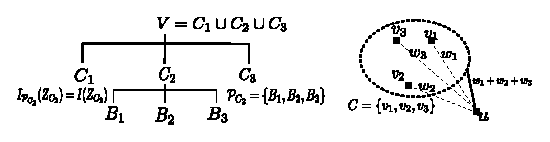
\includegraphics[width=\textwidth]{pic/two_approach.eps}
\caption{hierarchical tree generation based on multivariate similarity. Left figure shows the top-down approach with each subset split into multiple sets. Right figure shows the bottom-up approach with the graph nodes $v_1,v_2,v_3$ contracted to $C$. The weight between $C$ and node $u$ is $w_1+w_2+w_3$.}\label{fig:ta}
\end{figure}

By the construction of the clustering tree, we can associate each tree node with a threshold value, which is the multivariate similarity computed at that step.
\begin{example}
\begin{figure}
\centering
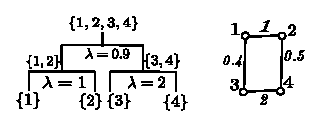
\includegraphics[width=0.7\textwidth]{pic/threshold.eps}
\caption{a clustering tree (left) for the weighted graph (right) by graph-based info-clustering method. Threshold values are $0.9, 1, 2$.}\label{fig:threshold}
\end{figure}
Consider an undirected graph $G(V, E)$ with $V=\{1,2,3,4\}$ and $E=\{(1,2),(1,3),(3,4),(2,4)\}$ with edge weight $w_{12}=1,w_{13}=0.4,w_{24}=0.5,w_{34}=2$ (See Fig. \ref{fig:threshold}). The threshold values are the multivariate similarity $I(Z_{3,4})=2, I(Z_{1,2})=1$ and $I(Z_V)=0.9$ respectively. We can write the complete clustering solution as:
\begin{equation*}
\P = 
\begin{cases}
\{\{1,2,3,4\}\} & \lambda < 0.9 \\
\{\{1,2\},\{3,4\}\} & 0.9 \leq \lambda < 1 \\
\{\{1\},\{2\},\{3,4\}\} & 1 \leq \lambda < 2\\
\{\{1\},\{2\},\{3\},\{4\}\} & \lambda \geq 2
\end{cases}
\end{equation*}
Although the clustering tree does not distinguish $\{\{1\},\{2\},\{3,4\}\}$ with $\{\{1,2\},\{3\}, \{4\}\}$, the partition $\{\{1,2\},\{3\}, \{4\}\}$ does not exist.
\end{example}
Using $I(Z_V)$ to cluster directly is computational expensive, the same clustering result can be achieved by solving the following optimization problem for all $\lambda$ (Corollary 2 in \cite{RN1}).
\begin{theorem}[Theorem 3.7 in \cite{RN3}]\label{thm:psp}
\begin{align}\label{eq:hL}
h_{\P}(\lambda) &=  f[\P] - \abs{\P} \lambda  \\
h(\lambda) &= \min_{\P \in \Pi'(V)} h_{\P}(\lambda)
\end{align}
The optimal partitions for $h(\lambda)$ are finite and they can be arranged in a decreasing sequence $\P_1, \dots, \P_k$ such that $\P_1 \succeq \P_2 \dots \succeq \P_k$, This sequence is called principal sequence of partitions of $h(\lambda)$ and we can obtain the hierarchical clustering tree from this sequence.
\end{theorem}
%proof in attachment

Since $h_{\P}(\lambda)$ is linear about $\lambda$, $h(\lambda)$ is piecewise linear and each turning point of $h(\lambda)$ corresponds to $\P_i, \P_{i+1}$ respectively. 

Info-clustering assumes that the weight is additive and tends to produce trivial hierarchical structure when the value of weights are near equal. This property is shown by the following theorem.
\begin{theorem}\label{thm:trival}
The partition to minimize equation \eqref{eq:ms} is $\P_k = \{\{1\},\{2\},\dots,\{\abs{V}\}\}$ if and only if equation \eqref{eq:GF} holds.
\begin{equation}\label{eq:GF}
\frac{f[\P]}{\abs{\P}-1} \geq \frac{f[\P_k]}{\abs{V}-1} \textrm{ for any } \P \in \Pi'
\end{equation}
\end{theorem}
\begin{proof}
We use Theorem \ref{thm:psp}. Since $h(\lambda)$ is piecewise linear, the first line segment of $h(\lambda)$ is $ - \lambda $ and the last line segment is $ f[\P_k] - \abs{V} \lambda$. Their intersection point is $(\lambda_{+}, -\lambda_{+})$ where $\lambda_{+} = \frac{f[\P_k]}{\abs{V}-1}$. Since $\frac{f[\P]}{\abs{\P}-1} \geq \lambda_{+} \iff f[\P] - \abs{\P}\lambda_{+} \geq - \lambda_{+}$ Equation \eqref{eq:GF} says the minimizer of $h(\lambda)$ at $\lambda = \lambda_{+}$ is either $\{V\}$ or $\{\{1\},\{2\},\dots,\{\abs{V}\}\}$ and $h(\lambda)$ has only two line segments. From geometric point of view, the solution to equation \eqref{eq:ms} is the first turning point of $h(\lambda)$ and it is equal to that of last turning point if and only if \eqref{eq:GF} holds.
\end{proof}
By Theorem \ref{thm:trival}, we can show that if all graph weights are of equal value, then by applying info-clustering we can only get trivial cluster $\{V\}$. Generally, we have the following proposition.
\begin{proposition}\label{prop:triangle}
Let $w_{ij}=0$ if $(i,j)\not\in E$. If $w_{ij} + w_{jk} \geq w_{ki}$ for any different triple $i, j, k \in V$, then the info-clustering solution is trivial\footnotemark.
\end{proposition}
\footnotetext{By trivial solution we mean only $\{V\}$ is a cluster, or the hierarchical tree contains only root and leaves.}

Proposition \ref{prop:triangle} inspires us in order to separate different clusters, we need small magnitude of inter-cluster weights and large similar intra-cluster weight.

\section{Algorithm}\label{sec:algorithm}

In this section, we review the basic theory to solve equation \eqref{eq:hL} and propose an improved algorithm flow (Fig. \ref{fig:pyramid}) based on the work of \cite{RN4}. 

Since $h(\lambda)$ is piecewise linear, we can use divide and conquer to search the turning points and evaluate $h(\lambda)$ only at these turning points. This is the method proposed at \cite{RN7} and has complexity $N^2 \mathtt{MaxFlow}(N)$ if the hierarchical tree structure is needed. 
%If we are only interested in finding a suitable partition  with at least $k$ part, then the algorithm complexity can be reduced to $\log(N) N \mathtt{MaxFlow}(N)$. This is the approach evaluated at subsection \ref{sec:fc}.

We call the above approach Dilworth truncation. It solves \eqref{eq:hL} for fixed $\lambda$  by solving the following problem sequentially for $t=1,\dots,\abs{V}$.
\begin{align}
\tilde{h}_{\lambda}(T) &= f(T) - \lambda - y^{\lambda}(T)\\
\tilde{h}(\lambda) & = \min_{t \in T \subseteq V} \tilde{h}_{\lambda}(T) \label{eq:pmq}
\end{align}
where
$y^{\lambda}_i = \min\{a_i - \lambda, b_i\}$  and $b_i \leq +\infty$. 

\begin{figure}
	\centering
	\begin{subfigure}{0.4\textwidth}
		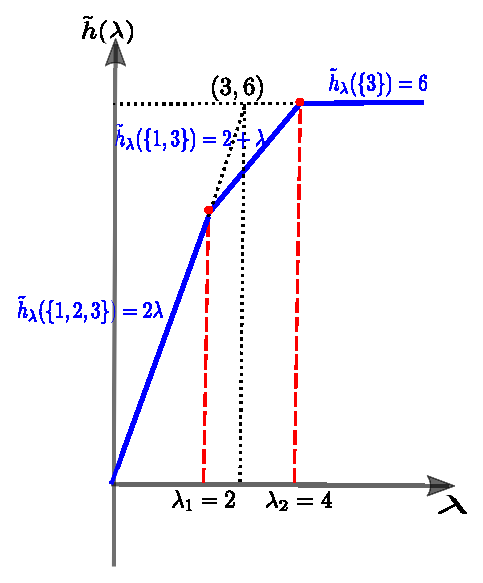
\includegraphics[width=\textwidth]{pic/example_pst_single.eps}
		\caption{An illustration of Algorithm \ref{alg:pmfT}}\label{fig:linseg}
	\end{subfigure}
	\begin{subfigure}{0.4\textwidth}
		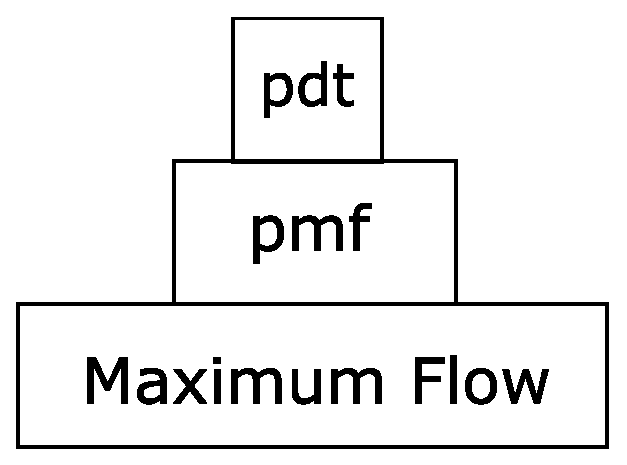
\includegraphics[width=\textwidth]{pic/pdt.eps}
		\caption{Algorithmic pyramid to compute principal sequence of partitions. The top level is parametric Dilworth truncation; the middle level is parametric maximum flow and the bottom level is maximum flow.}\label{fig:pyramid}
	\end{subfigure}
	\caption{Algorithm Illustration}
\end{figure}

It is pointed out in \cite{RN4} that equation \eqref{eq:pmq} can be solved with $\lambda$ as a parameter, not a value. We call this method parametric Dilworth truncation (\textsf{pdt} in short, in Fig \ref{fig:pyramid}). It can solve \eqref{eq:hL} directly by treating $\lambda$ as a parameter. However, solving \eqref{eq:pmq} for fixed $t$ is not a trivial task and the approach given in \cite{RN4} is quite complex to analyze. Below, we propose a clear and efficient approach to solve \eqref{eq:pmq} for $\lambda\geq 0$. 

First we have the following property to the solution set of $\tilde{h}(\lambda) $.
\begin{proposition}\label{prop:struc}
If $f$ is a submodular function which satisfies $f(A\cup B) + f(A\cap B) \leq f(A) + f(B)$ and 
let $A^{\lambda}$ be the solution to $\tilde{h}(\lambda)$, then 
\begin{equation}\label{eq:Alambda}
\mathcal{A}^{\lambda}=\begin{cases}
T_0 & \lambda < \lambda_1 \\
T_i & \lambda_i \leq \lambda < \lambda_{i+1}, \textrm{ for } i=1, 2, \dots, k-1 \\
T_k & \lambda \geq \lambda_{k}
\end{cases}
\end{equation}
where $T_k \subsetneq  \dots \subsetneq T_1 \subsetneq T_0$
\end{proposition}

In Proposition \ref{prop:struc}, if $\lambda$ is sufficiently large, then all $y_i^{\lambda}$ will have the form $a_i -  \lambda$ and the minimum solution is $\{t\}$. That is, $T_k = \{t\}$. On the other hand, since we are only concerned about $\lambda \geq 0$. We can compute \eqref{eq:pmq} for $\lambda = -\epsilon (\epsilon > 0)$. Then we have $T_0$ and $T_k$ in \eqref{eq:Alambda}.

Another important observation of function $\tilde{h}(\lambda)$ is that it is piecewise linear and concave. $T_0$ corresponds the first linear part and $T_k$ corresponds the last one.  To compute the nested family between $T_0$ and $T_k$, we use divide and conquer, which is presented in Algorithm \ref{alg:pmfT}.
\begin{algorithm}
	\caption{Parametric Computing of $T^{\lambda} = \argmin_{t\in V} g_{\lambda}(T)$}\label{alg:pmfT}
	\begin{algorithmic}[1]
		\REQUIRE set $V$, $t \in V$, function $g_{\lambda}$ whose domain is $V$.
		\ENSURE An ordered array \textbf{L} which contains $\lambda_1, \dots \lambda_k$ and a reversely ordered array $T^{\lambda}$ which contains $T_0,\dots, T_k$. (defined in equation \eqref{eq:Alambda})
		\STATE \textbf{L}, $A^{\lambda} \leftarrow$ empty arrays of size $\abs{V}$
		\STATE $Q \leftarrow \argmin_{A\in V} g_{-\epsilon}(A), P \leftarrow \{ t \}$ \label{alg:uini}
		\STATE add $Q$ and $P$ to $T^{\lambda}$
		\STATE \texttt{Split}$(Q,P)$
		\FUNCTION{\texttt{Split}$(Q,P)$}
		\STATE Let $\tilde{\lambda}_2$ be the solution to $g_{\lambda}(Q) =  g_{\lambda}(P)$
		\STATE $h' = g_{\tilde{\lambda}_2}(Q)$
		\STATE $P' =\argmin_{A\in V} g_{\tilde{\lambda}_2}(A)$  \label{alg:Pap}
		\IF{$ g_{\tilde{\lambda}_2}(P') = h'$}
		\STATE add  $\tilde{\lambda}_2$ to $\mathbf{L}$
		\ELSE
		\STATE add $P'$ to $T^{\lambda}$ \label{alg:addP}
		\STATE \texttt{Split}$(Q,P')$
		\STATE \texttt{Split}$(P',P)$
		\ENDIF
		\ENDFUNCTION
	\end{algorithmic}
\end{algorithm}

\begin{example}
We use the graph defined in Example \ref{eg:three} (Fig. \ref{fig:tn}) and define $f$ as the graph cut function, $t=3$ and $y^{\lambda}_i = -\lambda, i=1,2,3$. 
We can get $T_0 = \{1,2,3\} $ and $T_k = \{3\}$. And their corresponding lines are $\tilde{h}_{\lambda}(T_0) =2\lambda$ and $\tilde{h}_{\lambda}(T_k)=6$. As Fig. \ref{fig:linseg} shows, they intersect at $(3, 6)$; Since $\tilde{h}(3)=5<6$, the set $T_1=\{1,3\}$ from Algorithm \ref{alg:pmfT} line \ref{alg:addP}. That is, there are turning points of $\tilde{h}$ at interval $(0, 3)$ and $(3, +\infty)$ respectively. For $(0,3)$, we compute the intersection of $\tilde{h}_{\lambda}(T_0)$ and $\tilde{h}_{\lambda}(T_1)=1+\lambda$ and get the intersection coordinate $(1,2)$; Also $\tilde{h}(1)=2$, therefore  the computation for $(0,3)$ is finished. The same goes for $(3, +\infty)$. And finally, we can get $L=[1,5, +\infty]$ and $A^{\lambda} = [\{1,2,3\}, \{1,3\},\{3\}]$.	
\end{example}

Algorithm \ref{alg:pmfT} is only theoretically computable. To make it possible to implement, we need to figure out how to compute $\tilde{h}(\lambda)$ for given $\lambda$ efficiently.

To simplify our notation, in this section we will let $w_{ij} = 0$ if $(i,j) \not\in E$. To compute $\tilde{h}(\lambda)$, we combine Algorithm \ref{alg:pmfT} and the parametric maximum flow algorithm (shorted as \textsf{pmf} in Fig \ref{fig:pyramid}). The combination begins at creating a new weighted directed graph $\widetilde{G}(\widetilde{V}, \widetilde{E})$ from directed graph $G(V,E)$ by the following steps:
\begin{enumerate}
	\item Add a new node $s$ and initialize $c^{\lambda}(s,v)=\max\{0, -y^{\lambda}_v\}$ for $v \in V\backslash \{t\}$
	\item Copy the weight of $G$ to arc capacity of $\widetilde{G}$ and modify the in-arc capacity of node $t$ as $c^{\lambda}(v,t) = w_{vt} + \max\{0, y^{\lambda}_v\}$ for $ v \in V\backslash \{s\}$
	\end{enumerate}

\begin{figure}
	\centering
	\begin{subfigure}{0.33\textwidth}
		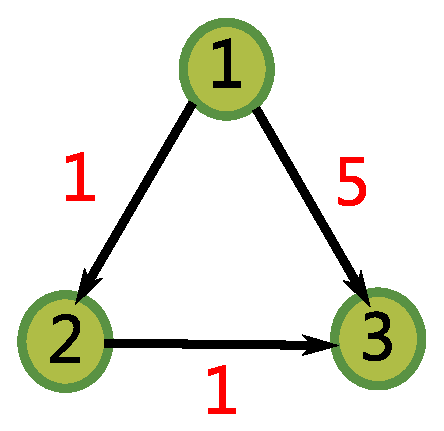
\includegraphics[width=\textwidth]{pic/example_directed.eps}
		\caption{a graph $G$ with three nodes}\label{fig:tn}
	\end{subfigure}~
	\begin{subfigure}{0.36\textwidth}
		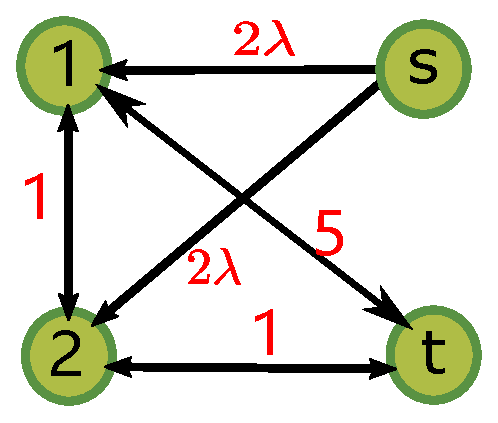
\includegraphics[width=\textwidth]{pic/example_st.eps}
		\caption{$\widetilde{G}$ derived from left graph with $t=3$}\label{fig:tn_converted}
	\end{subfigure}
	\caption{Example graph $G$ and its conversion to $\widetilde{G}$}
\end{figure}
For $\widetilde{G}(\widetilde{V}, \widetilde{E})$, there are two special nodes $s$ and $t$, The s-t cut for $\widetilde{G}$
is defined as $c^{\lambda}(T) = \sum_{i \not\in T, j \in T} c^{\lambda}(i,j)$ where $s \not\in T, t \in T$. By such construction we can guarantee $c^{\lambda}(i,j)\geq 0$ and have the following property:
\begin{theorem}\label{thm:constDiff}
	\begin{align}
		\tilde{h}_{\lambda}(T) &= c^{\lambda}(T) - \lambda - \sum_{v \in V} \max\{0, y^{\lambda}_v\}\\
	A^{\lambda}	&= \argmin_{s\in U\backslash T, t\in T}c^{\lambda}(T) \label{eq:pmqe}
	\end{align}
\end{theorem}
\begin{proof}
	
	\begin{align*}
	c^{\lambda}(T) &= f(T) + \sum_{i \not\in T} (c^{\lambda}(i, t) - w_{it})+ \sum_{j \in T} c^{\lambda}(s,j) \\
	\Rightarrow \tilde{h}_{\lambda}(T) - c^{\lambda}(T) &= -\lambda - \sum_{j \in T} y^{\lambda}_j - \sum_{i \not\in T} \max\{0, y^{\lambda}_i\} - \sum_{j \in T} \max\{0,-y^{\lambda}_j\}\\
	&= -\lambda - \sum_{v \in V} \max\{0, y^{\lambda}_v\}
	\end{align*}
\end{proof}

By Theorem \ref{thm:constDiff}, for a given $\lambda, \tilde{h}_{\lambda}$ and $c^{\lambda}$ differ a constant value for any $T\subseteq V$. Therefore, we can use $c^{\lambda}$ instead of $\tilde{h}_{\lambda}$ in Algorithm \ref{alg:pmfT} and $\argmin c^{\lambda}$ can be computed by maximum flow algorithm. 

Within function \texttt{Split} in Algorithm \ref{alg:pmfT}, an important note is that we do not compute $P'$ in line \ref{alg:Pap} freshly but starting from a given flow map which is obtained from the maximum flow map after computing $Q$. By doing so, the time complexity can be significantly reduced.

Algorithm \ref{alg:pmfT} is invoked $\abs{V}$ times by iterating $t=1,\dots \abs{V}$. By the analysis in \cite{RN17}, the time complexity for \textsf{pmf} can be achieved with the same of maximum flow. If the highest label selection rule is used, the overall time complexity for parametric Dilworth truncation is $O(\abs{V}^3\sqrt{\abs{E}})$ \cite{RN9}. Compared with those iterative method whose number of iteration is controlled by accuracy $\epsilon$, graph-based info-clustering method terminates in strongly polynomial time.

\section{Experiment}\label{sec:experiment}
In this section, we demonstrate graph-based info-clustering on two kinds of problems. The first is about data clustering, in which we need to cluster multi-dimensional vectors. For this kind of task, we need to construct the clustering graph first by using a proper similarity measure. The other problem is community detection and the sample graph is coming from \cite{RN22}, in which a two-level hierarchical structure is defined. By comparison with other clustering methods, we will show that graph-based info-clustering gives reasonable good result and can recover the two-level hierarchical structure under certain conditions. 

\subsection{Data Clustering}\label{sec:fc}
For data clustering task, we prepare three groups of data, coming from \cite{RN7}:
\begin{enumerate}
\item Four Gaussian blobs with unit variance and centers at $(3,3), (3,-3), (-3,3), (-3,-3)$ respectively.  We generate 25 points for each blob.
\item Three concentric circles with radius $0.1,0.2,0.3$ and number of data points as $60, 100, 140$. The angles of these points are uniform distributed and they also oscillate along the radius direction.
\item UCI glass dataset with 214 samples, 6 classes, 9 dimensions of feature.
\end{enumerate}
We use adjusted rand index as the metric to score different clustering method, the best performance for each algorithm is shown in Table \ref{tb:e1}.  It can be seen from the table that graph-based info-clustering is better than other clustering algorithms.
\begin{table}[!ht]
\centering
\InputIfFileExists{compare_3.tex}{}{}
\caption{ accuracy for different clustering algorithms }\label{tb:e1}
\end{table}
\subsection{Community Detection}
\begin{figure}
	\centering
	\begin{subfigure}{0.45\textwidth}
		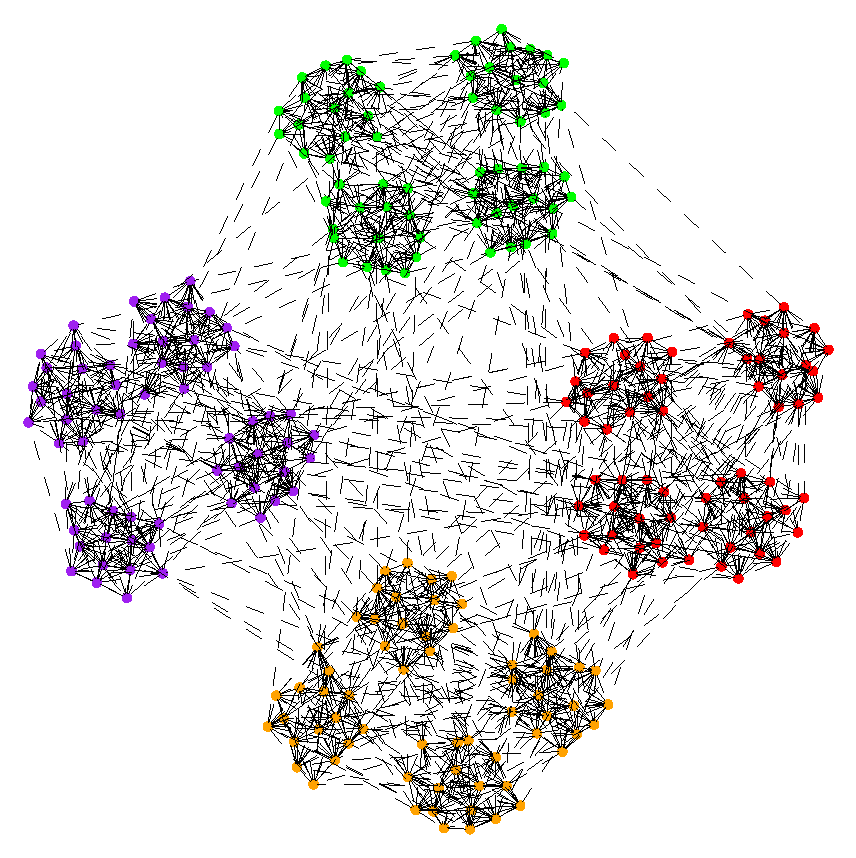
\includegraphics[width=\textwidth]{pic/two_level.eps}
		\caption{a community with two hierarchical levels with $z_{\mathrm{in}_1} = 14,$ $z_{\mathrm{in}_2} = 3, z_{\mathrm{out}}=1$.}\label{fig:c1}
	\end{subfigure}
	\begin{subfigure}{0.45\textwidth}
		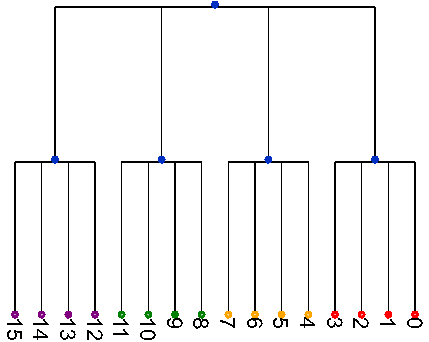
\includegraphics[width=\textwidth]{pic/tree_info-clustering.pdf}
		\caption{hierarchical tree obtained by graph-based info-clustering for left figure. The tree leaves with the same ancestor are merged for clarity.}\label{fig:c2}
	\end{subfigure}
	\caption{Community Detection Experiment Illustration}
\end{figure}

For the community detection task, we use a two-level artificial dataset proposed in \cite{RN22}. 
The community structure is shown in Fig. \ref{fig:c1}. It has 4 communities in macro-level, and each macro community contains 4 micro communities. We use $z_{\mathrm{in}_1}$ to represent the internal average degree of nodes within micro community; $z_{\mathrm{in}_2}$ as node degree between different micro communities but within one macro community; $z_{\mathrm{out}}$ as node degree between different macro communities. By varying one and fixing the other two in $\{z_{\mathrm{in}_1}, z_{\mathrm{in}_2}, z_{\mathrm{out}} \}$ we get different set of experiment. To compare the deduced hierarchical tree structure with the ground truth, we use the normalized Robinson-Foulds distance as the metric. It describes the distance between two trees with different topology and falls within $[0,1]$. We compare the RF distance of graph-based info-clustering with that of GN (Girvan-Newman algorithm) and BHCD (a Bayesian Hierarchical method in \cite{RN23}). The result is shown in Fig. \ref{fig:cdr}. As can be seen from Fig.\ref{fig:cdr}, in either case, graph-based info-clustering can produce more similar tree structures than that of the ground truth.
\begin{figure}
	\centering
	\begin{subfigure}{0.33\textwidth}
		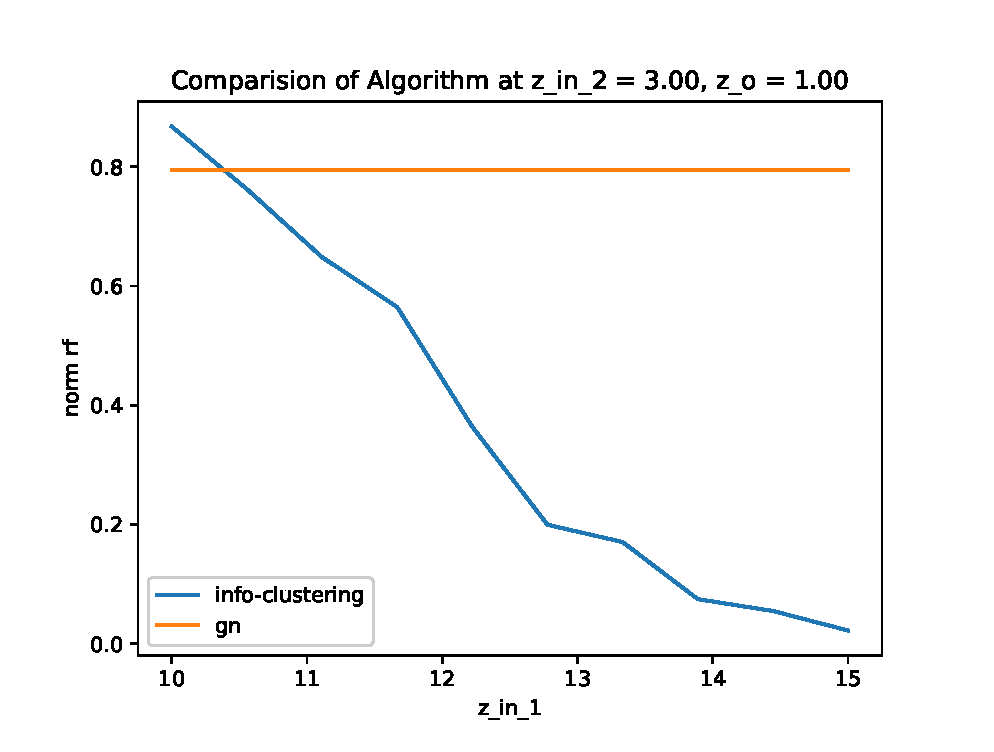
\includegraphics[width=\textwidth]{pic/z_in_1.eps}
		\caption{}
	\end{subfigure}~
	\begin{subfigure}{0.33\textwidth}
		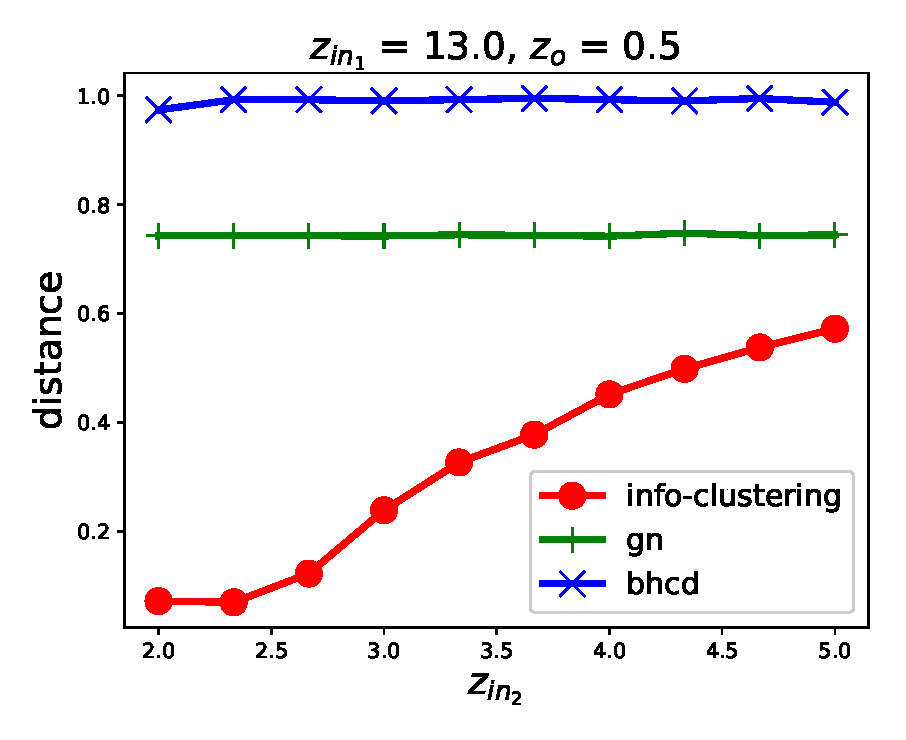
\includegraphics[width=\textwidth]{pic/z_in_2.eps}
		\caption{}
	\end{subfigure}~
	\begin{subfigure}{0.33\textwidth}
		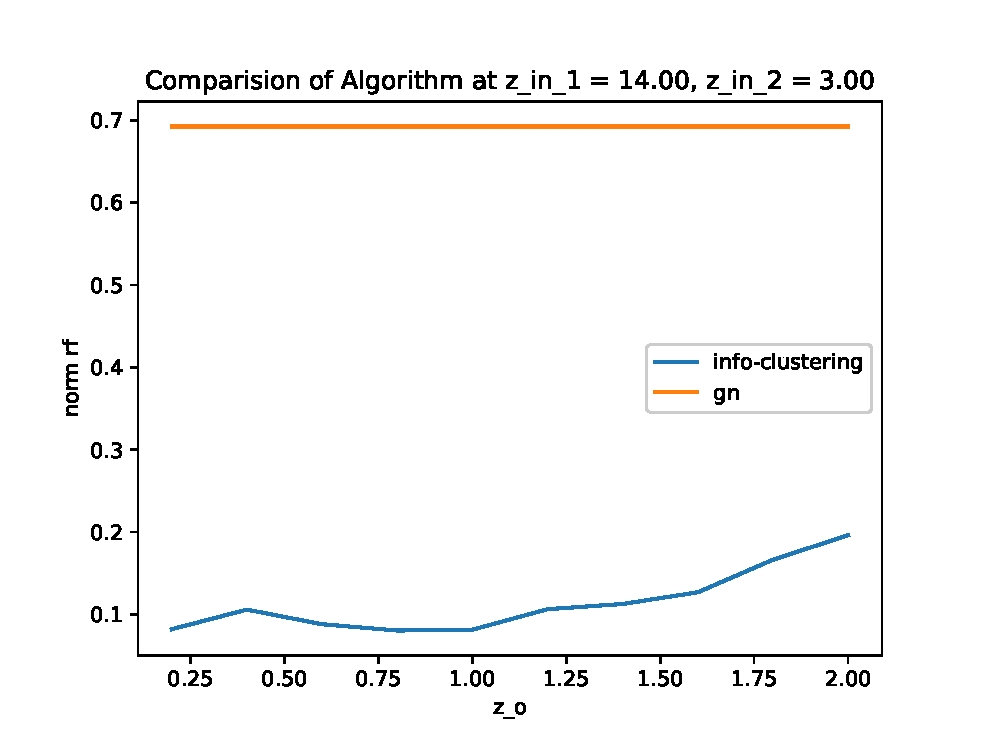
\includegraphics[width=\textwidth]{pic/z_o.eps}
		\caption{}
	\end{subfigure}
	\caption{Distance comparison between different hierarchical community detection method. Smaller distance indicates more similar structure with the ground truth tree.}\label{fig:cdr}	
\end{figure}

For such problems with unweighted graph, it is more practical to give weight values for graph-based info-clustering by 
\begin{equation}
    w_{ij} = 1 + \abs{\{k | (i,k),(j,k) \in E \}} \textrm{ for } (i,j) \in E
\end{equation}
This weight assignment scheme is the number of triangles which contain the edge and can be justified by the following proposition.

\begin{proposition}\label{prop:reweight}
Suppose $S_1, S_2 $ are complete graph node set with $\abs{S_1}=\abs{S_2}=n$ and equal weight $w_{ij}=n$. There are $m$ edges between the two graphs and all inter-connection edges have equal weight 1. Then for $V=S_1\cup S_2$, we have
\begin{equation}
I(Z_V) = \begin{cases}
m & m <\frac{n^2}{2}, S_1,S_2 \textrm{ are non-trival cluster} \\
\frac{m+n^2(n-1)}{2n-1} & m\geq \frac{n^2}{2}, \textrm{ only trival cluster\footnotemark exists} 
\end{cases}
\end{equation}
\end{proposition}
\footnotetext{$V$ is a trival cluster.}

Proposition \ref{prop:reweight} tells us there is no other clusters except for $S_1$ and  $S_2$. It inspires us to increase the weight linearly with the number of nodes for densely connected part of the whole community. It improves the clustering results of graph-based info-clustering.



\section{Conclusion}\label{sec:conclusion}
In this paper, we formulate info-clustering in graph theory language and propose a parametric computing scheme to efficiently get the hierarchical structure of dataset or community. Numerical experiments show that graph-based info-clustering performs well and is especially suitable if the tree structure of ground truth is far different from the binary tree structure.

%\subsubsection*{Acknowledgments}



\bibliographystyle{plain}
\bibliography{exportlist}


\end{document}
